% CHAPITRE 1 — Diagnostic et Analyse de l'Existant (5-6 pages)

\chapter{Diagnostic et Analyse de l'Existant}
\label{ch:diagnostic}

Ce chapitre présente l'environnement professionnel dans lequel s'est déroulé le stage, analyse la procédure existante de dépôt et de traitement des plaintes, et identifie le besoin auquel la plateforme PlainteCam doit répondre.

Il procède en cinq temps. La première section décrit la structure d'accueil, son positionnement et son organisation. La deuxième rend compte de l'audit conduit sur le terrain, en reconstituant la procédure manuelle telle qu'elle est réellement pratiquée et en relevant les difficultés qui s'y attachent. La troisième examine les dispositifs comparables déjà déployés ailleurs, en France, au Sénégal et au Cameroun même. La quatrième synthétise ces constats dans une analyse SWOT. La cinquième en tire l'expression du besoin auquel la solution devra répondre.

\section{Présentation de l'entreprise Access Finance \& RH SARL}

La structure d'accueil est présentée ici sous cinq angles : son positionnement, son implantation, sa mission, ses domaines d'activité et son organisation interne.

\subsection{Historique et positionnement}

Access Finance \& RH SARL est une entreprise spécialisée dans le développement de solutions numériques sur mesure à destination des organisations publiques et privées. Fondée avec pour ambition de répondre aux défis croissants de la transformation digitale, l'entreprise a développé une expertise reconnue dans la conception d'applications web, l'intégration de systèmes d'information et le déploiement de solutions métier innovantes.

L'entreprise se positionne comme un acteur incontournable dans son domaine, combinant expertise technique et connaissance approfondie du contexte institutionnel de ses clients. Access Finance \& RH SARL accompagne ses partenaires depuis la phase d'analyse des besoins jusqu'à la mise en production et la maintenance des solutions déployées.

\subsection{Localisation et implantation}

Access Finance \& RH SARL est stratégiquement implantée pour servir efficacement sa clientèle locale et régionale. L'entreprise dispose d'installations modernes équipées des technologies nécessaires au développement de logiciels de pointe.

\begin{figure}[H]
    \center
    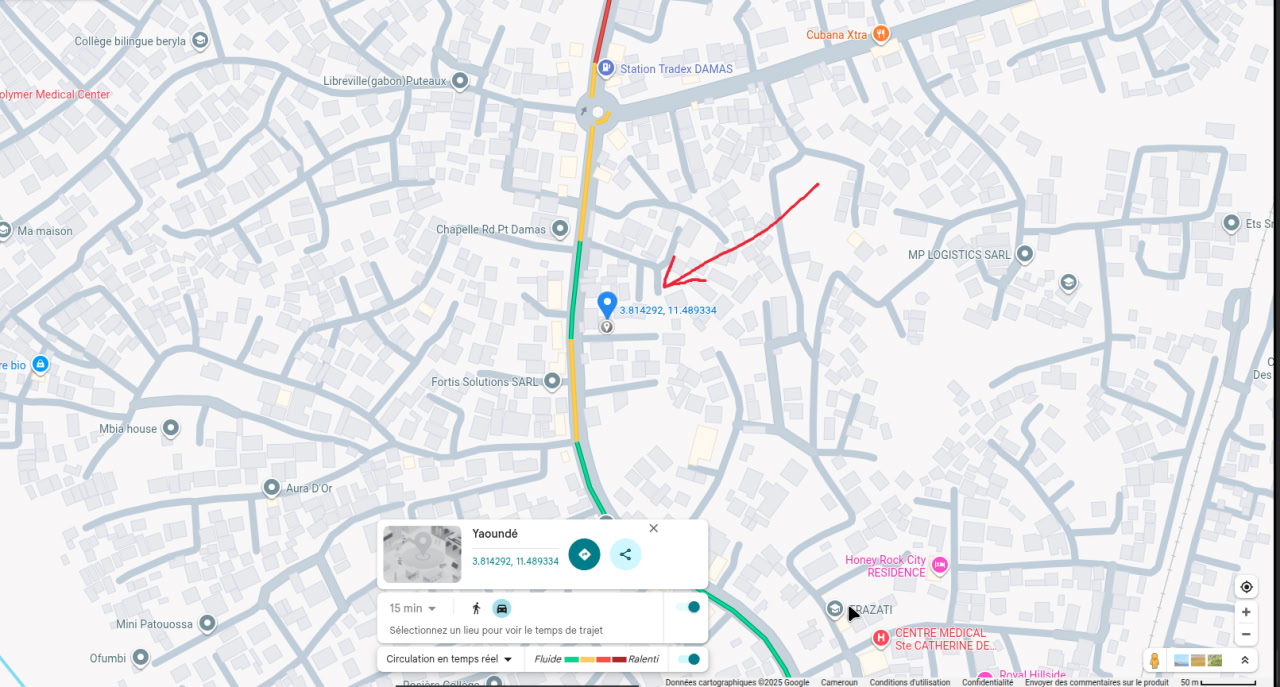
\includegraphics[width=0.68\textwidth, height=6.8cm]{images/localisation.jpg}
    \caption{Localisation géographique de Access Finance \& RH SARL}
    \label{fig:localisation}
\end{figure}

\subsection{Mission et vision}

\textbf{Mission :} Access Finance \& RH SARL analyse les besoins de ses clients, propose des solutions numériques adaptées et pilote leur déploiement dans le respect des délais, de la qualité et des coûts.

\textbf{Vision :} Devenir le partenaire de référence des organisations dans leur transformation numérique et l'optimisation de leurs processus métier.

\subsection{Domaines d'activité}

Access Finance \& RH SARL structure son offre autour de trois axes. Le \textbf{développement d'applications sur mesure} conduit les clients du cahier des charges à la mise en production : applications web, plateformes métier et systèmes d'information adaptés à chaque organisation. Le \textbf{conseil et l'audit numérique} portent sur l'évaluation des systèmes existants et la formulation de recommandations d'optimisation. Enfin, la \textbf{maintenance et le support} garantissent, par contrat, la continuité de service et l'évolution des solutions déployées.

\subsection{Organigramme}

Access Finance \& RH SARL fonctionne avec une structure resserrée, caractéristique des entreprises de services numériques à taille humaine : les circuits de décision sont courts et chaque intervenant couvre un périmètre large. L'organisation s'articule autour des rôles suivants :

\begin{itemize}
    \item \textbf{Direction générale}, assurée par la dirigeante de l'entreprise : orientation stratégique, relation avec les clients institutionnels et arbitrages d'engagement sur les projets.
    \item \textbf{Direction technique (CTO)} : définition des choix d'architecture et de technologies, garantie de la qualité des livrables et encadrement de l'équipe de production.
    \item \textbf{Tech Lead}, chargé du pilotage technique au quotidien : découpage des tâches, revues de code, accompagnement des développeurs et interface avec la direction technique.
    \item \textbf{Équipe de développement} : un développeur senior, référent sur les projets les plus complexes, et les développeurs chargés de l'implémentation des solutions.
    \item \textbf{Design UX/UI} : maquettage des écrans, ergonomie des parcours et cohérence visuelle des interfaces livrées.
    \item \textbf{Équipe commerciale} : prospection, réponse aux consultations et suivi de la relation client.
\end{itemize}

Le présent stage s'est déroulé au sein de l'\textbf{équipe de développement}, sous la supervision de l'encadreur professionnel, avec des points réguliers auprès du Tech Lead pour les choix de conception.

\begin{figure}[H]
    \centering
    \centerline{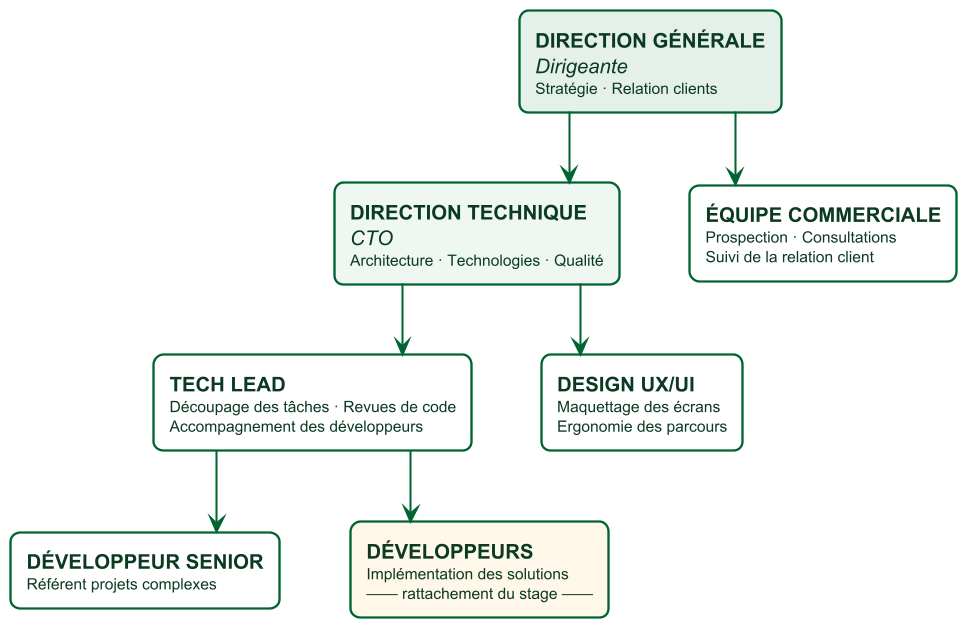
\includegraphics[width=0.80\linewidth]{diagrammes/organigramme_klivar.png}}
    \caption{Organigramme de l'entreprise Access Finance \& RH SARL}
    \label{fig:organigramme}
\end{figure}

\section{Analyse de la situation existante}

Cette section retrace d'abord le déroulement de la mission, puis restitue la procédure de dépôt et de traitement des plaintes telle que l'audit de terrain l'a documentée, avant d'en relever les difficultés.

\subsection{Déroulement du stage et missions effectuées}

Mon intégration au sein de Access Finance \& RH SARL s'est déroulée de manière progressive. Dès les premiers jours, j'ai été présenté aux différents pôles de l'entreprise. Mon maître de stage, M.~\textbf{NDJON MBOG THIERRY}, a encadré l'ensemble de la mission avec rigueur et disponibilité.

La mission s'est déroulée en cinq phases sur les six mois du stage. Les \textbf{deux premières semaines} ont été consacrées à l'audit et à l'analyse de l'existant : observation de la procédure aux commissariats de Ngoa-Ekélé et de Mimboman, entretiens avec les personnels et identification des points de friction. Les \textbf{deux semaines suivantes} ont porté sur la conception de la solution, avec la définition de l'architecture, la modélisation UML et le maquettage des interfaces. Du \textbf{deuxième au quatrième mois} s'est étendu le développement de PlainteCam, couvrant l'implémentation du frontend, celle du backend et l'intégration de l'intelligence artificielle. Le \textbf{cinquième mois} a été réservé aux tests et à la validation : recette fonctionnelle, corrections et validation par les parties prenantes. Le \textbf{sixième et dernier mois} a été employé à la documentation et à la rédaction du présent mémoire.

\subsection{Description de la procédure manuelle actuelle}

L'audit a été conduit dans deux commissariats de Yaoundé, celui de \textbf{Ngoa-Ekélé} et celui de \textbf{Mimboman}, selon une approche qualitative semi-directive : des entretiens avec des fonctionnaires de police de ces unités, menés sur guide structuré et anonymisés pour favoriser la franchise des réponses, complétés par l'observation directe du flux de travail sur place : réception des plaignants, circulation des dossiers papier, gestion des parafeurs. Le recours à deux unités distinctes permettait de distinguer ce qui relève de la procédure commune de ce qui tient aux habitudes propres à un service. La procédure reconstituée ci-dessous s'articule en quatre temps.

\subsubsection*{Réception et enregistrement}

Le plaignant se présente au commissariat \textbf{territorialement compétent}, c'est-à-dire celui du secteur où réside le mis en cause ou celui où les faits ont eu lieu, le maillage des unités étant fixé par l'organisation de la Sûreté nationale. Sa plainte doit obligatoirement comporter la date, ses nom et adresse, l'objet de la plainte, l'identité du mis en cause et la destination de l'acte, commissaire ou procureur. Le secrétariat enregistre la plainte et la transmet au chef d'unité. Une \textbf{attestation de dépôt} est délivrée au plaignant et jointe au dossier : elle constitue la preuve officielle qu'il a bien porté plainte.

\subsubsection*{Cotation à un enquêteur}

Le chef d'unité \textbf{cote} ensuite la plainte à un enquêteur, lequel reçoit un \textbf{parafeur} regroupant l'ensemble des dossiers dont il a la charge. Le critère retenu est la compétence de l'enquêteur sur le type d'affaire concerné, mais \textbf{aucune procédure n'est formalisée} : l'arbitrage repose sur la connaissance qu'a le chef d'unité de son équipe. En cas d'indisponibilité de l'enquêteur désigné, le dossier est transféré à un autre.

\subsubsection*{Auditions et procès-verbaux}

Le plaignant est convoqué puis auditionné, et un \textbf{procès-verbal} est dressé. Le mis en cause est convoqué à son tour et auditionné, donnant lieu à un second procès-verbal. Lorsqu'il est identifié, il est convoqué \textbf{au minimum trois fois} ; en cas d'absence répétée et injustifiée, le dossier est transmis au procureur.

La rédaction des procès-verbaux est \textbf{entièrement manuscrite}. L'enquêteur transcrit à la main les déclarations en suivant un \textbf{template institutionnel} normalisé : en-tête (commissariat, date, heure, numéro de dossier), identité complète de la personne auditionnée, corps de la déclaration, questions et réponses le cas échéant, clôture et mentions légales.

\subsubsection*{Convocation et suivi}

Un point particulier est apparu déterminant lors de l'entretien : c'est \textbf{en principe le plaignant lui-même qui remet la convocation au mis en cause}. Un policier ne l'assiste que s'il redoute des représailles. Quant au suivi, il n'existe \textbf{aucun dispositif} : pour connaître l'état d'avancement de son dossier, le plaignant doit se déplacer au commissariat.

\begin{figure}[H]
    \centering
    
\includegraphics[width=0.72\textwidth]{images/problematique_flux.png}
    \caption{Flux de traitement manuel : points de friction identifiés}
    \label{fig:flux_manuel}
\end{figure}

Cette procédure ne laisse \textbf{aucune trace numérique}. Il en découle une conséquence que l'audit a jugée centrale : le délai qui sépare le dépôt de la cotation, comme celui du traitement complet d'une affaire, \textbf{n'est mesuré nulle part}. Il varie selon l'affluence, la nature des faits et la disponibilité des enquêteurs, et seul le commissariat en a une appréciation empirique. Ce n'est donc pas la longueur des délais qui constitue le problème documenté, mais l'\textbf{impossibilité de les connaître}, et par conséquent de les piloter.

\subsection{Difficultés et limites identifiées lors de l'audit}

L'entretien a permis de recenser quatre difficultés récurrentes, qui tiennent moins à l'organisation du service qu'aux situations concrètes rencontrées au guichet et en salle d'audition.

La première tient à l'\textbf{analphabétisme d'une partie des plaignants}, qui ne savent ni lire ni écrire et doivent être assistés par une personne de leur choix. La procédure s'en trouve ralentie, le plaignant devient dépendant d'un tiers, et la confidentialité de sa déclaration s'en trouve fragilisée.

La deuxième tient à la \textbf{difficulté d'exposer les faits de façon claire et ordonnée}. Beaucoup de plaignants racontent par fragments, dans le désordre, en omettant des éléments qu'ils jugent secondaires. Il en résulte un dossier incomplet et un procès-verbal lacunaire.

La troisième, et l'entretien l'a présentée comme la plus contentieuse, est le \textbf{refus du mis en cause de signer le procès-verbal} dont il conteste la fidélité. Elle ouvre un contentieux procédural et fait peser un risque de vice de forme sur la suite de l'affaire.

La quatrième tient à la \textbf{rédaction manuscrite des procès-verbaux}, longue et répétitive. Elle représente une charge administrative lourde, et ce temps est directement soustrait au travail d'enquête proprement dit.

À ces difficultés s'ajoutent trois limites structurelles relevées par l'observation : le \textbf{déplacement obligatoire} pour déposer comme pour s'informer, l'\textbf{absence de traçabilité} interdisant tout audit et toute mesure, et la \textbf{remise de la convocation par le plaignant lui-même}, qui fait peser sur la victime une démarche potentiellement risquée.

Il est notable que trois de ces quatre difficultés, les points 1 à 3, concernent la \textbf{qualité et la valeur juridique de la déclaration} plutôt que la lenteur du circuit. Ce constat a orienté la conception : la solution devait d'abord fiabiliser le recueil des faits, et non se contenter d'accélérer la circulation des dossiers.

\section{Ce qui existe ailleurs}

Avant d'envisager un développement, il fallait vérifier qu'aucune solution existante ne répondait déjà au besoin. Trois dispositifs comparables ont été examinés.

En \textbf{France}, le dispositif de pré-plainte a laissé place, en octobre 2024, à une \textbf{plainte en ligne} de plein exercice, doublée d'un service de visioconférence dénommé \textit{Visioplainte}~\cite{france-visioplainte}. Le plaignant y dépose sa plainte sans se déplacer, s'entretient à distance avec un officier, puis reçoit le procès-verbal par voie électronique et le confirme avant signature par l'agent. Ce dispositif demeure toutefois réservé aux \textbf{atteintes aux biens dont l'auteur est inconnu} : les faits commis contre les personnes, comme ceux dont l'auteur est identifié, en restent exclus, au motif qu'ils peuvent justifier une intervention immédiate.

Au \textbf{Sénégal}, la police nationale a mis en service en février 2026 une \textbf{plateforme de signalement des infractions cybercriminelles}~\cite{senegal-psic}. Elle permet de dénoncer en ligne, de manière sécurisée et confidentielle, les escroqueries commises sur internet, le cyberharcèlement, l'usurpation d'identité ou les atteintes aux données personnelles. Son périmètre est donc \textbf{thématique} : il ne couvre que la délinquance numérique, et le dispositif s'arrête au signalement, sans prendre en charge l'instruction qui doit suivre.

Au \textbf{Cameroun} enfin, la Délégation générale à la sûreté nationale a engagé en 2022, avec l'appui de la coopération allemande, un projet de plateforme numérique destinée au traitement automatisé des plaintes des usagers~\cite{cameroun-dgsngiz}. Son objet est cependant \textbf{distinct du nôtre} : il s'agit de recueillir les plaintes \emph{dirigées contre la police}, dans une logique de contrôle interne, et non de permettre à une victime de déposer une plainte pénale. Le numéro vert qui remplissait auparavant cette fonction était du reste jugé peu efficace par le public.

Deux enseignements se dégagent de cette comparaison. D'abord, les dispositifs existants sont \textbf{restreints} : soit par la nature des faits (atteintes aux biens, cyberinfractions), soit par la qualité de l'auteur, qui doit demeurer inconnu. Ensuite, ils s'arrêtent au \textbf{dépôt} ou au signalement : aucun ne prend en charge la suite de la chaîne, c'est-à-dire la cotation à un enquêteur, la conduite des auditions, la rédaction des procès-verbaux et l'émission des convocations.

Aucun de ces dispositifs ne traite les difficultés relevées lors de notre audit : un plaignant qui ne sait ni lire ni écrire, une convocation remise par la victime elle-même, une cotation sans procédure formalisée. Ces constats justifient le développement d'une solution propre plutôt que la reprise d'un outil existant.

Le dispositif français mérite toutefois d'être retenu comme \textbf{piste d'évolution} : en faisant dialoguer la victime avec un officier par visioconférence, il apporte au problème de l'illettrisme une réponse que PlainteCam traite autrement, par la dictée vocale et le questionnaire guidé. Les deux approches sont complémentaires plutôt que concurrentes.

\section{Analyse SWOT liée à la mission}

Le service observé ne part pas de rien. Ses \textbf{forces} ne sont d'ailleurs ni techniques ni matérielles : elles sont humaines et juridiques. Il dispose de personnels formés, rompus à la conduite des auditions et à la qualification juridique des faits ; d'une connaissance fine du terrain, que les entretiens menés dans les deux commissariats ont confirmée ; d'un maillage territorial d'unités déjà établi et connu des habitants ; enfin d'un cadre de procédure stable, qui désigne sans ambiguïté qui peut dresser un procès-verbal et dans quelles formes.

Ses \textbf{faiblesses} tiennent au support de la procédure, non aux personnes qui l'appliquent. Le dossier circule sur papier, aucun système d'information ne le suit, et l'absence de trace numérique interdit non seulement l'audit mais toute mesure : ni le délai de cotation ni celui du traitement complet ne sont connus. La hiérarchie ne dispose donc d'aucun élément objectif pour répartir la charge entre ses enquêteurs, ni pour rendre compte de l'activité de son unité.

Deux évolutions extérieures constituent aujourd'hui des \textbf{opportunités} qui n'existaient pas hier : la maturité des technologies web, qui permet de livrer un service utilisable depuis un terminal modeste et une connexion instable, et l'accessibilité de l'intelligence artificielle générative, dont certains modèles s'obtiennent désormais sans engagement financier. S'y ajoute le taux d'équipement mobile des citoyens, sans lequel un dépôt en ligne resterait une hypothèse d'école.

Les \textbf{menaces} sont de deux ordres. Les premières pèsent sur le service tel qu'il fonctionne : la perte de confiance de citoyens lassés de se déplacer sans obtenir d'information, et l'égarement ou l'altération de dossiers que rien ne duplique. Les secondes naîtraient du projet lui-même : la résistance au changement de personnels attachés à des pratiques éprouvées, et surtout la contestation de la valeur probante d'un dossier constitué par voie numérique.

C'est le \textbf{croisement} de ces facteurs qui a orienté la conception, davantage que leur inventaire. Le cadre juridique stable, porté au rang des forces, est précisément ce qui désarme la menace la plus sérieuse : un dossier numérique demeure défendable tant que le procès-verbal reste l'acte de l'officier de police judiciaire, ce qui exclut toute validation automatique. La faiblesse la plus lourde, des délais que personne ne mesure, trouve dans la maturité des technologies web une réponse immédiate, l'horodatage de chaque transition. Quant au maillage territorial, il cesse d'être un simple actif pour devenir le socle du rattachement automatique au commissariat compétent : la cascade géographique ne fait que rendre calculable une organisation déjà en place.

\section{Identification du besoin}

Les constats qui précèdent convergent vers une même conclusion, qu'il reste à formuler explicitement avant d'aborder la conception.

\subsection{Pourquoi les méthodes actuelles ne suffisent plus}

L'analyse de l'existant a mis en évidence quatre problèmes fondamentaux qui rendent la procédure actuelle insuffisante :

\textbf{Un problème d'accessibilité :} Le déplacement au commissariat constitue une barrière significative, en particulier pour les personnes éloignées, à mobilité réduite ou craignant de se présenter en personne. Il réduit le nombre de plaintes effectivement déposées et alourdit inutilement le parcours du citoyen.

\textbf{Un problème de fiabilité du recueil :} La qualité du dossier dépend de la capacité du plaignant à exposer les faits et de la retranscription qu'en fait l'agent. Un plaignant illettré, intimidé ou peu à l'aise à l'oral produit une déclaration lacunaire, que la rédaction manuscrite du procès-verbal ne permet ni de compléter ni de contrôler méthodiquement.

\textbf{Un problème de sécurité pour le plaignant :} La remise de la convocation au mis en cause incombe en principe à la victime elle-même. Cette exposition directe, dans une affaire où l'auteur présumé est souvent un proche ou un voisin, peut dissuader de poursuivre la procédure, voire de la déclencher.

\textbf{Un problème de traçabilité :} L'absence de système d'information centralisé empêche tout suivi par le plaignant, tout audit a posteriori et toute mesure de l'activité du service. Faute d'horodatage, le commissariat ne dispose d'aucun élément objectif pour arbitrer l'affectation de ses moyens ni pour rendre compte de son activité.

Trois contraintes encadrent la réponse à apporter. La première est juridique : le procès-verbal demeure un acte de l'officier de police judiciaire, et aucun dispositif automatique ne peut s'y substituer~\cite{cameroun-cpp}. La deuxième tient à la confidentialité : un dossier de plainte n'est consultable que par son plaignant, l'enquêteur qui en a la charge et sa hiérarchie. La troisième est matérielle : la plateforme doit rester utilisable depuis un terminal mobile d'entrée de gamme et une connexion instable.

Enfin, une réserve de périmètre doit être posée d'emblée : la contestation par le mis en cause du contenu de son procès-verbal relève de la procédure, non du logiciel. La plateforme peut en conserver la trace horodatée, elle ne peut pas l'empêcher. Il ne sera donc pas prétendu qu'elle résout cette difficulté.
